\documentclass[]{IEEEtran}

% Your packages go here
\usepackage[utf8]{inputenc}
\usepackage{graphicx}

\markboth{MC949/MO446 Computer Vision}{}

\begin{document}
  \title{Your awesome title}
  \author{Leonardo Rezende, Thales Oliveira (RA 148051) and Iury 
    \thanks{-, t148051@dac.unicamp.br, -}
  }
  \maketitle
  
  \begin{abstract}
    In this project the group was able to get in contact with the development environment to be worked with during the Computer Vision Course. The exercises proposed were completed, and the manipulated images are shown throughout this report. By resolving the problems, the group was able to work with OpenCV and related libraries for image manipulation in the Python programming language.
  \end{abstract}
  
  \section{Introduction}
  
  This work, developed by Group 8 of Computer Vision Course (2nd Semester/2019), has the objective of introducing the tools used in the field of Computer Vision, and also to practice programming skills needed to succeed in the following projects. The theme of the exercises is basic image manipulation using OpenCV library, and the group decided to work with the Python programming language. The project consists of 5 exercises, divided by specific parts. The solutions of each question, which can be output images, text answers or both, are listed in the next section (Image outputs and Answers). The Conclusion section sums up the work done. 


  \section{Image outputs and Answers}
  \subsection{Exercise 1}
  For this exercise, it was supposed to find an image to be used as input for the next exercises. The chosen image is displayed in figure \ref{fig:i-1-0}, and it is 300x400 pixels, in order to fit the requirements.
  \begin{figure}[!h]
    \centering
    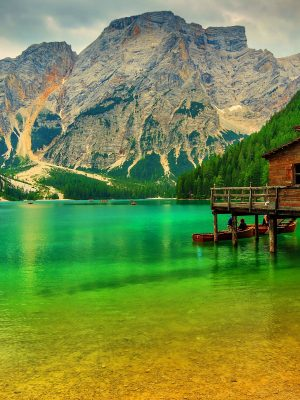
\includegraphics{../input/i-1-0.jpg}
    \caption{Image input used for exercises 2 to 5}
    \label{fig:i-1-0}
  \end{figure}

  actions and work goes here.
  
  \section{Conclusion}
  
  You conclude your work here.
  
\end{document}